% Required packages in preamble:
% \usepackage{tikz}
% \usetikzlibrary{trees}
% \usepackage{xcolor}

% Define styles for readability
\tikzset{
  box/.style={thick, minimum size=1cm, draw, align=center},
  less/.style={box, fill=green!20},
  pivot/.style={box, fill=red!20},
  greater/.style={box, fill=blue!20},
  tree/.style={level distance=1.2cm, sibling distance=2.2cm, grow=down, every node/.style={font=\small}},
}

% Frame: Pivot Selection
\begin{frame}{Quicksort Step: Select Pivot}
  \centering
  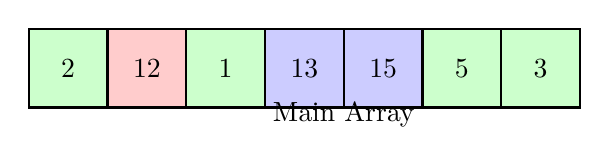
\begin{tikzpicture}
    \foreach \val/\color [count=\i from 0] in {2/less, 12/pivot, 1/less, 13/greater, 15/greater, 5/less, 3/less} {
        \node[\color] at (\i, 0) {\val};
      }
    \node[below=6pt] at (3.5, -0.1) {Main Array};
  \end{tikzpicture}

  \vspace{1em}
  \textbf{Pivot index:} 1 \\
  \textbf{Pivot value:} 12
\end{frame}

% Frame: Partitioning
\begin{frame}{Quicksort Step: Partitioning}
  \centering
  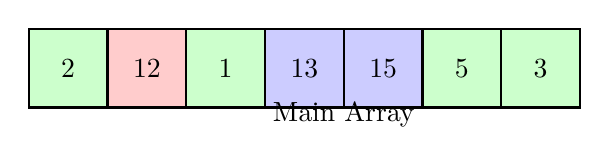
\begin{tikzpicture}
    \foreach \val/\color [count=\i from 0] in {2/less, 12/pivot, 1/less, 13/greater, 15/greater, 5/less, 3/less} {
        \node[\color] at (\i, 0) {\val};
      }
    \node[below=6pt] at (3.5, -0.1) {Main Array};
  \end{tikzpicture}

  \vspace{1em}
  \textbf{Partition:} \\
  \textcolor{green!50!black}{Left: 2, 1, 5, 3} \\
  \textcolor{red}{Pivot: 12} \\
  \textcolor{blue}{Right: 13, 15}
\end{frame}

% Frame: Recursion Tree
\begin{frame}{Quicksort Recursion Tree}
  \begin{center}
    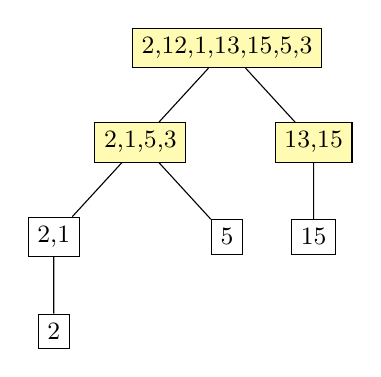
\begin{tikzpicture}[tree]
      \node[draw, fill=yellow!30]{2,12,1,13,15,5,3}
      child { node[draw, fill=yellow!30]{2,1,5,3}
          child { node[draw]{2,1}
              child { node[draw]{2} }
            }
          child { node[draw]{5} }
        }
      child { node[draw, fill=yellow!30]{13,15}
          child { node[draw]{15} }
        };
    \end{tikzpicture}
  \end{center}
\end{frame}

% Frame: Base Cases
\begin{frame}{Quicksort Base Cases}
  \centering
  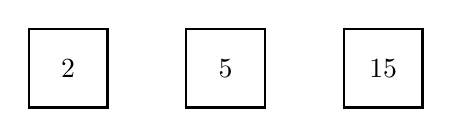
\begin{tikzpicture}
    \node[box] at (0, 0) {2};
    \node[box] at (2, 0) {5};
    \node[box] at (4, 0) {15};
  \end{tikzpicture}

  \vspace{1em}
  Arrays 2, 5, and 15 are already sorted.
\end{frame}
